\chapter{Results}
\todoa{Find diffusion for one atom?}

\section{Density}
\begin{figure}[htpb]%
    \centering%
    \includesvg[width=0.7\textwidth, svgpath=./images/density/]{density_water02}%
    \caption{%
        Density of water. \hl{FINISH CAPTION, normalize against bulk density}. %
%         \label{fig:cell_lists}%
    }%
\end{figure}%

\begin{figure}[htpb]%
    \centering%
    \includesvg[width=0.7\textwidth, svgpath=./images/density/]{density_water03}%
    \caption{%
        Density of water. \hl{FINISH CAPTION, normalize against bulk density}. %
%         \label{fig:cell_lists}%
    }%
\end{figure}%

\begin{figure}[htpb]%
    \centering%
    \includesvg[width=0.7\textwidth, svgpath=./images/density/]{number_of_molecules02}%
    \caption{%
        Number of molecules. Bin width = 0.2 \AA?. \hl{FINISH CAPTION}. %
%         \label{fig:cell_lists}%
    }%
\end{figure}%

\begin{figure}[htpb]%
    \centering%
    \includesvg[width=0.7\textwidth, svgpath=./images/density/]{density_water_normalized02}%
    \caption{%
        Density of water. %
%         \label{fig:cell_lists}%
    }%
\end{figure}%

\begin{figure}[htpb]%
    \centering%
    \includesvg[width=0.7\textwidth, svgpath=./images/density/]{density_water_normalized03}%
    \caption{%
        Density of water. %
%         \label{fig:cell_lists}%
    }%
\end{figure}%

\FloatBarrier
\section{Diffusion/mean square displacement}
\todoa{Measure diffusion with move origin for better statistics}
\todob{Fix footnotesize stuff in diffusion figures}
\todo[inline]{Diffusion normal to and parallel to surface?}
\begin{figure}[htpb]%
    \centering%
    {
        \newcommand{\f}{\footnotesize}
        \includesvg[width=0.7\textwidth, svgpath=./images/diffusion/]{diffusion01}%
    }
    \caption{%
        Diffusion. \hl{Make new figure using new diffusion program}. %
%         \label{fig:cell_lists}%
    }%
\end{figure}%

% \begin{figure}[htpb]%
%     \centering%
%     {
%         \newcommand{\f}{\footnotesize}%
%         \includesvg[width=0.7\textwidth, svgpath=./images/diffusion/]{diffusion_constant02}%
%     }
%     \caption{%
%         Diffusion. \hl{Make new figure using new diffusion program} \hl{FINISH CAPTION}. %
% %         \label{fig:cell_lists}%
%     }%
% \end{figure}%

\begin{figure}[htpb]%
    \centering%
    \includesvg[width=0.7\textwidth, svgpath=./images/diffusion/]{diffusion_constant_move_origin01}%
    \caption{%
        Diffusion. \hl{FINISH CAPTION}. %
%         \label{fig:cell_lists}%
    }%
\end{figure}%

\begin{figure}[htpb]%
    \centering%
    \includesvg[width=0.7\textwidth, svgpath=./images/diffusion/]{diffusion_constant_move_origin02}%
    \caption{%
        Diffusion. \hl{FINISH CAPTION}. %
%         \label{fig:cell_lists}%
    }%
\end{figure}%

\begin{figure}[htpb]%
    \centering%
    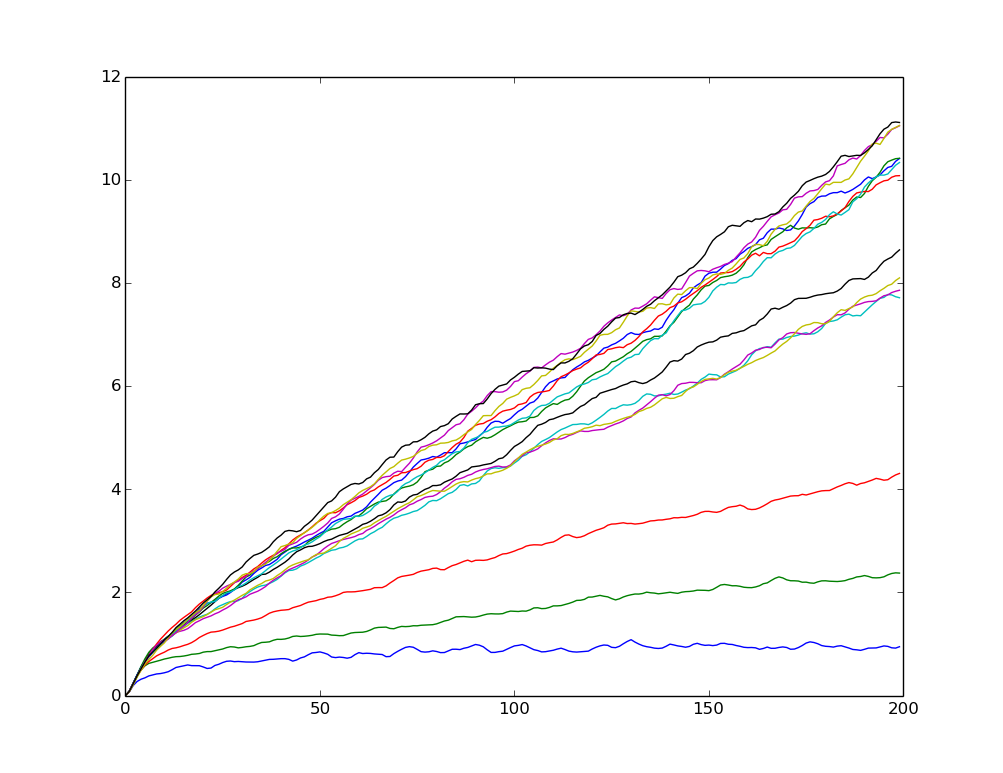
\includegraphics[width=0.7\textwidth]{images/diffusion/mean_square_displacement_interesting.png}%
    \caption{%
        Something interesting (msd stops increasing for a couple of angstrom near 4.5-5, 5-5.5, 5.5-6.0) \hl{FINISH CAPTION}. %
%         \label{fig:cell_lists}%
    }%
\end{figure}%

\FloatBarrier
\section{Distance to atom}
\todo{replace these with results from actual fracture system?}
We developed a program that finds the distance to the nearest atom, in all points of the 
%
\setlength{\myfigwidth}{0.90\textwidth}%
\begin{figure}[htpb]%
    \centering%
    \includesvg[pretex=\normalsize, width=\myfigwidth, svgpath = ./images/distance_to_atom/]{SiO2_06_slice_r05_n256}%
    \caption{$r = 5$ \Ang}%
    \label{fig:distance_to_atom_r05}%
\end{figure}%
%
\begin{figure}[htpb]%
    \centering%
    \includesvg[pretex=\normalsize, width=\myfigwidth, svgpath = ./images/distance_to_atom/]{SiO2_06_slice_r20_n256}%
    \caption{$r = 20$ \Ang}%
    \label{fig:distance_to_atom_r20}%
\end{figure}%

\FloatBarrier
\section{``Generation matrix''}
\todo{replace these with results from actual fracture system?}
Not very useful. Much of the same as distance to atom, only worse (but faster).
%
\begin{figure}[htpb]%
    \centering%
    \includesvg[pretex=\normalsize, width=\myfigwidth, svgpath = ./images/generation_matrix/]{SiO2_06_slice_r05_n256}%
    \caption{5 generations}%
    \label{fig:generation_matrix_r05}%
\end{figure}%
%
\begin{figure}[htpb]%
    \centering%
    \includesvg[pretex=\normalsize, width=\myfigwidth, svgpath = ./images/generation_matrix/]{SiO2_06_slice_r11_n256}%
    \caption{11 generations}%
    \label{fig:generation_matrix_r11}%
\end{figure}%
%
\begin{figure}[htpb]%
    \centering%
    \includesvg[pretex=\normalsize, width=\myfigwidth, svgpath = ./images/generation_matrix/]{SiO2_06_slice_r40_n256}%
    \caption{40 generations}%
    \label{fig:generation_matrix_r40}%
\end{figure}%

\FloatBarrier
\section{Tetrahedral order parameter}
\todoa{Make two separate TOP figures, one for regular rough, and one for rough with same surfac x2 ?}
% %
% \begin{figure}[htpb]%
%     \centering%
%     \includesvg[width=1.0\textwidth, svgpath = ./images/tetrahedral_order_parameter/]{fancyfig04}%
%     \caption{}%
% %     \label{fig:distance_to_atom_r20}%
% \end{figure}%
%
% \begin{figure}[htpb]%
%     \centering%
%     \includesvg[%
% %         width=\textwidth,% choose which fits best, width or height (regular includegraphics can use both and add "keepaspectratio", but includesvg can't)
%         height=\textheight,%
%         svgpath = ./images/tetrahedral_order_parameter_new/]{figure01}%
%     \caption{\hl{Caption, add legends!}}%
% %     \label{fig:distance_to_atom_r20}%
% \end{figure}%
%
\begin{figure}[htpb]%
    \centering% 
    \includesvg[%
%         width=\textwidth,% choose which fits best, width or height (regular includegraphics can use both and add "keepaspectratio", but includesvg can't)
        height=\textheight,%
        svgpath = ./images/tetrahedral_order_parameter_new/%
    ]{figure01_thin_fractures}%
    \caption{}%
%     \label{fig:distance_to_atom_r20}%
\end{figure}%
%
\begin{figure}[htpb]%
    \centering%
    \includesvg[%
%         width=\textwidth,% choose which fits best, width or height (regular includegraphics can use both and add "keepaspectratio", but includesvg can't)
        height=\textheight,%
        svgpath = ./images/tetrahedral_order_parameter_new/%
    ]{figure01_normal_fractures}%
    \caption{}%
%     \label{fig:distance_to_atom_r20}%
\end{figure}%

\FloatBarrier
\section{Area}
\section{Volume?}

